\documentclass[../notes.tex]{subfiles}

\pagestyle{main}
\renewcommand{\chaptermark}[1]{\markboth{\chaptername\ \thechapter\ (#1)}{}}
\renewcommand{\thechapter}{\Roman{chapter}}
\setcounter{chapter}{4}

\begin{document}




\chapter{Coordination Chemistry: Structures and Isomers of Metal Complexes}
\section{Module 28: Introduction to Coordination Compounds}
\begin{itemize}
    \item \marginnote{2/12:}Modern inorganic chemistry is heavily concerned with the transition metals, i.e., the $d$-block elements.
    \begin{itemize}
        \item Most industrial catalysts utilize transition metal compounds.
    \end{itemize}
    \item Transition metals vs. main-group elements:
\end{itemize}
\begin{tchart}{1.4}{Transition-Metal Compounds}{Main-Group Elements}
    Multiple oxidation states (e.g., the 11 oxidation states of \ce{Mn} from $-3$ to $+7$) & Single oxidation state\\
    Brightly colored (thus a gap between HOMO and LUMO of a few electron volts) & Usually colorless\\
    Usually have partially occupied valence $d$-orbitals that are often relatively close in energy & The valence $s$- or $p$-orbitals are either fully occupied or empty and are far apart energetically\\
    Often paramagnetic & Usually diamagnetic\\
    Often interact with small molecules such as \ce{CO}, \ce{C2H4}, and \ce{H2} & Generally do not interact strongly with  \ce{CO}, \ce{C2H4}, or \ce{H2}
\end{tchart}
\begin{itemize}
    \item The orbital energy gap matches the bond energies of small molecules pretty well.
    \begin{itemize}
        \item This is exactly what is needed for activating those chemical bonds, i.e., making catalytic cycles!
    \end{itemize}
    \item History:
    \begin{itemize}
        \item Prussian blue ink is the first synthetic blue dye, and one of the first coordination compounds created (used in famous paintings such as \emph{Starry Night}).
        \item The structure of coordination complexes was not understood until 1907, however.
        \item Blomstrand and Jorgenson tried to determine the structure of \ce{Co(NH3)4Cl3}, but their guess didn't explain isomers.
        \item Alfred Werner (late 1800s) was the father of coordination chemistry.
        \begin{itemize}
            \item He noticed that excess \ce{AgNO3} could only liberate and precipitate as \ce{AgCl} one chlorine from both the green and violet isomers of \ce{CoCl3*(NH3)4}.
            \item However, it could precipitate two chlorines from \ce{CoCl3*(NH3)5} and three from \ce{CoCl3*(NH3)6}.
            \item This observation plus a number of controls led him to \textbf{Werner's Conclusions}.
        \end{itemize}
    \end{itemize}
    \item \textbf{Werner's Conclusions}:
    \begin{enumerate}
        \item In this series of compounds, cobalt has a constant \textbf{coordination number} of 6.
        \item As the \ce{NH3} molecules are removed, they are replaced by \ce{Cl-}, which acts as if it is covalently bonded to cobalt.
        \item Chloride and ammonia are now called ligands.
        \item Ligands are a Lewis base/electron pair donors that can bind to a metal ion.
        \item A metal complex is a metal ion combined with ligands.
        \item Coordination complexes are neutral and counter ions are not bonded to the central metal ion but balance the charge.
        \begin{itemize}
            \item For example, in $[\stackrel{+3}{\ce{Co}}\!(\stackrel{0}{\ce{NH3}})_6]\!\stackrel{-3}{\ce{Cl}}_3$, the three chloride ions are the counter ions.
        \end{itemize}
    \end{enumerate}
    \item \textbf{Coordination number}: The number of groups that can bond directly to the metal.
    \item Werner also hypothesized an octahedral geometry for all cobalt complexes.
    \begin{itemize}
        \item If it were hexagonal planar or trigonal antiprismatic, there would be three isomers of the coordination sphere for the compound with two chlorines (think ortho, meta, para isomers for the hexagonal planar example).
        \item However, if it is octahedral, the compound with two chlorines will have two isomers (the chlorines can either be $\ang{180}$ to each other or $\ang{90}$ to each other).
        \item Octahedral also reduces steric crowding.
    \end{itemize}
    \item \textbf{Coodination compound}: A compound with a metal center, a coordination sphere, and counter ions. \emph{Also known as} \textbf{coordination complex}.
    \item Werner also resolved hexol into optically active isomers. This was the first optically active chiral \emph{inorganic} compound.
\end{itemize}



\section{Module 29: Types and Classes of Ligands}
\begin{itemize}
    \item \textbf{Monodentate ligand}: A ligand that binds to a metal ion through a single donor site. \emph{Etymology} one-toothed.
    \begin{itemize}
        \item For example, \ce{NH3} is a monodentate ligand.
    \end{itemize}
    \item \textbf{Bridging ligand}: A ligand that binds to two or more metal ions simultaneously.
    \begin{itemize}
        \item For example, \ce{O^2-} is a bridging ligand.
    \end{itemize}
    \item \textbf{Ambidentate ligand}: A ligand with two kinds of binding sites that can bind through one or the other but not both simultaneously.
    \begin{itemize}
        \item For example, thiocyanide can bond through \ce{S} or \ce{N} but not both simultaneously.
    \end{itemize}
    \item \textbf{Multidentate chelating ligand}: A ligand bound to a metal through several donor sites. \emph{Etymology} multitooth crab claw (crabs grab their food with two claws in the same way a metal can be attracted to two lone pairs from different groups on the same ligand). \emph{Also known as} \textbf{polydentate chelating ligand}.
    \begin{figure}[H]
        \centering
        \chemfig[atom sep=1cm]{[:54]M*5(-[,,,1,stealth-,grx,semithick]NH_2-[,,,1]CH_2-H_2C-[,,2,2]H_2N-[,,,,-stealth,grx,semithick])}
        \caption{An example of a bidentate chelating ligand.}
        \label{fig:bidentateLigand}
    \end{figure}
    \begin{itemize}
        \item For example, ethylenediamine (\ce{H2NCH2CH2NH2}; see Figure \ref{fig:bidentateLigand}) can bond to the same metal with both of its nitrogens' lone pairs at the same time.
        \item Thus, ethylenediamine is is bidentate, and it forms a 5-membered chelate ring.
    \end{itemize}
    \item The chelate effect: For a given metal ion, the thermodynamic stability of a chelated complex involving bidentate or polydentate ligands is greater than that of a complex containing a corresponding number of comparable monodentate ligands.
    \begin{itemize}
        \item Note that 5-membered rings are more stable than 6, and 4-membered rings (or smaller) are not stable due to angle strain.
        \item For example, ethylenediaminetetraacetate (EDTA) is a hexadentate ligand has two nitrogens and four oxygens that wrap entirely around a metal atom and bond very strongly.
        \item $\beta$-diketones and acetylacetone are also polydentate ligands.
        \item Multidentate bonding is incredibly strong.
        \item As one last example, hemoglobin and chlorophyll have extra stability because the iron/magnesium ion is attached to four nitrogens.
    \end{itemize}
    \item Explanations of the chelate effect:
    \begin{itemize}
        \item Effective concentration: If one bond breaks, the bridge between the two bonding sites in the ligands still holds the other site in close proximity to the metal, making it more likely that the bond will reform than if the metal and ligand were floating entirely independently.
        \item Entropy considerations:
        \begin{itemize}
            \item Imagine you have a coordination complex. If you substitute two monodentate ligands for two other monodentate ligands, you do not change the number of particles.
            \item However, if you substitute one polydentate chelating ligand for two monodentate ligands, you increase the number of particles by 1, increasing disorder in the universe and favoring the forward reaction.
        \end{itemize}
        \item Looking at the temperature-dependence of equilibrium, we can calculate $\Delta G^\circ$. We can then use this to calculate $\Delta H$ and $\Delta S$, and we find that the contributions are very similar. Thus, both explanations of the chelate effect contribute about equally.
    \end{itemize}
    \item Covalent bond classification (CBC) method:
    \item \textbf{X-type} (ligand): A ligand that donates one electron to the metal and accepts one electron from the metal when using the neutral ligand method of electron counting, or donates two electrons to the metal when using the donor pair method of electron counting.
    \begin{itemize}
        \item Examples: hydrogen, the halogens, hydroxide, cyanide, carbocation, and nitric oxide.
    \end{itemize}
    \item \textbf{L-type} (ligand): A neutral ligand that donates two electrons to the metal center regardless of the electron counting method being used.
    \begin{itemize}
        \item Examples: carbon monoxide, \ce{PR3}, ammonia, water, carbenes (\ce{=CRR}'), and alkenes.
    \end{itemize}
    \item \textbf{Z-type} (ligand): A ligand that accepts two electrons from the metal center as opposed to the donation occurring with the other two types of ligands.
    \begin{itemize}
        \item Examples: Lewis acids, such as \ce{BR3}.
    \end{itemize}
    \item LXZ notation:
    \begin{itemize}
        \item Take the traditional formula and replace the central metal atom with \ce{M}, each X-type ligand with \ce{X}, each L-type ligand with \ce{L}, and each Z-type ligand with \ce{Z}. Then, if necessary, combine ligands of the same type using subscript arabic numerals, as per usual. Conserve the braces and charge.
        \item For example, \ce{[Ir(CO)(PPh3)2(Cl)(NO)]^2+} becomes \ce{[ML3X2]^2+}.
    \end{itemize}
\end{itemize}



\section{Module 30: Nomenclature and Isomers of Metal Complexes}
\begin{itemize}
    \item \marginnote{2/15:}Midterm 1:
    \begin{itemize}
        \item Average: 67.0.
        \item Standard deviation: 14.8.
        \item Max: 93.
        \item $80+$ scores: 10.
    \end{itemize}
    \item Midterm 2 will cover modules 13-31 (with concepts from modules 1-12).
    \item Suggested reading: \textcite{bib:MiesslerFischerTarr} Section 9.2.
    \item Naming metal complexes:
    \begin{enumerate}
        \item For complex ions, write the cation first and anion last.
        \begin{itemize}
            \item For example, \ce{K2[PtCl4]} is potassium tetrachloroplatinate.
            \item Note that you do not use the prefix mono, di, tri, etc. here to indicate the number of cations.
        \end{itemize}
        \item Name the ligands first in alphabetical order, the metals last.
        \item Prefixes to indicate numbers (di, tri, tetra, \dots) for all monoatomic ligands, polyatomic ligands with short names and neutral ligands with special names.
        \item Prefixes bis-, tris-, tetrakis-, pentakis-, hexakis- for ligands whose names contain a prefix of the first type, neutral ligands without special names, and ionic ligands with particularly long names.
        \item If the anion is complex, add the suffix -ate to the name of the metal. If the symbol comes from Latin/Greek, then we go back to the Latin/Greek for the name of the anion.
        \item Put the oxidation state in Roman numerals in parentheses after the name of the central metal ion of the ligand.
    \end{enumerate}
    \item Examples:
    \begin{itemize}
        \item \ce{[CoCl4]^2-} is the tetrachlorocobaltate (II) ion.
        \item \ce{[Fe(CN)6]^4-} is the hexacyanoferrate (II) ion.
        \begin{itemize}
            \item Notice the use of "ferr" for iron (this is going back to the Latin/Greek name of the central metal ion as in Step 5).
        \end{itemize}
        \item \ce{[Cr(H2O)4Cl2]+} is the tetraaquodicchlorochromium (III) ion.
        \begin{itemize}
            \item No use of -ate because this is a cation (not an anion).
        \end{itemize}
        \item \ce{[Cr(NH2CH2CH2NH2)3]^3+} is the tris(ethylenediammine)chromium (III) ion.
        \begin{itemize}
            \item Note that ammine with two m's is correct --- an \textbf{amine} is a functional group from ammonia, while an \textbf{ammine} is a group of coordination compounds where ammonia is a ligand.
        \end{itemize}
    \end{itemize}
    \item Neutral ligands have the same name as the molecule with 4 exceptions:
    \begin{itemize}
        \item \ce{NH3} is ammine.
        \item \ce{H2O} is aquo.
        \begin{itemize}
            \item Aquo or aqua?
        \end{itemize}
        \item \ce{CO} is carbonyl.
        \item \ce{NO} is nitrosyl.
    \end{itemize}
    \item Anionic ligands require replacing -ide in the ionic name (if present) with -o. For example:
    \begin{itemize}
        \item \ce{Cl-} becomes chloro.
        \item \ce{OH-} becomes hydroxo.
        \item \ce{SO4^2-} is still sulfate.
    \end{itemize}
    \item Bridging ligands:
    \begin{figure}[H]
        \centering
        \chemleft{[}
            \chemfig{\ce{(H3N)4}Co^{III}(-[:-30,1.5]\chembelow{N}{\hspace{1.5mm}H_2}?)-[1]O-O-[7]Co^{III}\ce{(NH3)4}?}
        \chemright{]^{2-}}
        \caption{A coordination compound with bridging ligands.}
        \label{fig:muLigandNomenclature}
    \end{figure}
    \begin{itemize}
        \item Use $\mu$ to indicate a bridge.
        \item If there are more than one of a given bridging ligand, the prefix indicating the number of ligands is placed after the $\mu$.
        \item If there are more than one different bridging ligands, they are given in alphabetical order.
        \item For example, the compound in Figure \ref{fig:muLigandNomenclature} is the tetraaminecobaltate(III)-$\mu$-amido-$\mu$-peroxo-tetraaminecobaltate(III) ion.
    \end{itemize}
    \begin{table}[h!]
        \centering
        \renewcommand{\arraystretch}{1.4}
        \small
        \begin{tabular}{lll}
            \textbf{Common Name} & \textbf{IUPAC Name} & \textbf{Formula}\\
            \hline
            nitrido & nitrido & \ce{N^3-}\\
            azido & azido & \ce{N3-}\\
            oxo & oxido & \ce{O^2-}\\
            thiocyano & thiocyanato-S & \ce{SCN-}\\
            isothiocyano & thiocyanato-N & \ce{NCS-}\\
            thiocarbonyl & thiocarbonyl & \ce{CS}\\
            nitro & nitrito-N & \ce{NO2-}\\
            nitrito & nitrito-O & \ce{ONO-}\\
            phosphine & phosphane & \ce{PR3}\\
            pyridine & pyridine (abbrev. \ce{py}) & \ce{C5H5N}\\
            amido & azanido & \ce{NH2-}\\
            imido & azanediido & \ce{NH^2-}\\
        \end{tabular}
        \caption{Irregular and unfamiliar monodentate ligands.}
        \label{tab:irregularLigands}
    \end{table}
    \item Table \ref{tab:irregularLigands} lists some more common but irregular or unfamiliar ligands.
    \begin{itemize}
        \item Note that when listed in Table \ref{tab:irregularLigands}, ambidentate ligands bind through the atom listed most to the left in the formula.
        \item Note also that the slides list a number of common bidentate and polydentate ligands.
    \end{itemize}
    \item Suggested reading: \textcite{bib:MiesslerFischerTarr} Section 9.3.
    \item Coordination complex isomers are divided into:
    \begin{itemize}
        \item Structural isomers (different bonds).
        \begin{itemize}
            \item Coordination isomerism.
            \item Linkage isomerism.
        \end{itemize}
        \item Stereoisomers (same bonds, different spatial arrangements).
        \begin{itemize}
            \item Geometric isomerism (\emph{cis}-\emph{trans}).
            \item Optical isomerism.
        \end{itemize}
    \end{itemize}
    \item \textbf{Ionization isomers}: Ligands inside the coordination sphere exchange places with ligands outside the coordination sphere.
    \begin{itemize}
        \item So named because these give different ions when dissolved in water.
        \item Werner's four isomers of \ce{CrCl3*6H2O} are ionization isomers.
    \end{itemize}
    \item \textbf{Linkage isomers}: Variations in at which site an ambidentate ligand bonds.
    \item \textbf{Geometric isomers}: Found in square planar and octahedral complexes --- \emph{cis}- vs. \emph{trans}-isomers.
    \begin{figure}[h!]
        \centering
        \begin{subfigure}[b]{0.4\linewidth}
            \centering
            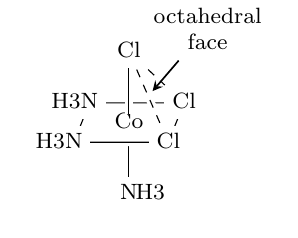
\begin{tikzpicture}[
                every node/.append style={black,fill=white,text height=1.5ex,text depth=0.25ex}
            ]
                \footnotesize
                \node (M) {Co};
                \draw (M) -- ++(0,-0.9) node[label={[xshift=-2.4mm]right:\ce{H3}}]{\ce{N}};
                \draw [white,very thick,double=black,double distance=0.4pt]
                    (-0.7,-0.25) node[label={[xshift=2.4mm]left:\ce{H3}}]{\ce{N}}
                    -- (0.5,-0.25) node(ClE1){\ce{Cl}}
                    -- (0.7,0.25) node(ClE2){\ce{Cl}}
                    -- (-0.5,0.25) node[label={[xshift=2.4mm]left:\ce{H3}}]{\ce{N}}
                    -- cycle
                ;
                \draw [white,very thick,double=black,double distance=0.4pt] ([yshift=-1mm]M.north) -- (M) -- ++(0,0.9) node(ClA){\ce{Cl}};

                \draw [white,very thick,double=black,double distance=0.4pt,dashed] (ClA) -- (ClE1) (ClA) -- (ClE2);
                \node (of) [align=center] at (1,1) {octahedral\\face} (of.210) edge [semithick,-stealth] (0.3,0.4);
            \end{tikzpicture}
            \caption{fac-triamminetrichlorocobalt(III).}
            \label{fig:facMera}
        \end{subfigure}
        \begin{subfigure}[b]{0.4\linewidth}
            \centering
            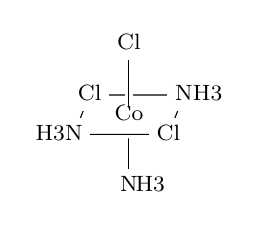
\begin{tikzpicture}[
                every node/.append style={black,fill=white,text height=1.5ex,text depth=0.25ex}
            ]
                \footnotesize
                \node (M) {Co};
                \draw (M) -- ++(0,-0.9) node[label={[xshift=-2.4mm]right:\ce{H3}}]{\ce{N}};
                \draw [white,very thick,double=black,double distance=0.4pt]
                    (-0.7,-0.25) node[label={[xshift=2.4mm]left:\ce{H3}}]{\ce{N}}
                    -- (0.5,-0.25) node{\ce{Cl}}
                    -- (0.7,0.25) node[label={[xshift=-2.4mm]right:\ce{H3}}]{\ce{N}}
                    -- (-0.5,0.25) node{\ce{Cl}}
                    -- cycle
                ;
                \draw [white,very thick,double=black,double distance=0.4pt] ([yshift=-1mm]M.north) -- (M) -- ++(0,0.9) node{\ce{Cl}};
            \end{tikzpicture}
            \caption{mer-triamminetrichlorocobalt(III).}
            \label{fig:facMerb}
        \end{subfigure}
        \caption{Facial and meridional geometric isomers.}
        \label{fig:facMer}
    \end{figure}
    \begin{itemize}
        \item Be aware of \textbf{facial} (fac) vs. \textbf{meridional} (mer) geometric isomers.
        \item In Figure \ref{fig:facMera}, all three \ce{Cl-Co-Cl} bond angles are $\ang{90}$.
        \item In Figure \ref{fig:facMerb}, two \ce{Cl-Co-Cl} bond angles are $\ang{90}$, and the other is $\ang{180}$.
    \end{itemize}
    \item Note that there are several different ways to represent an octahedrally coordinated metal ion.
    \begin{figure}[h!]
        \centering
        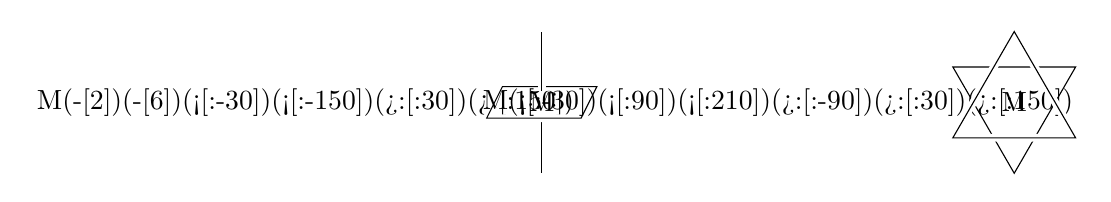
\begin{tikzpicture}
            \begin{scope}[xshift=-3cm]
                \node{\chemfig{M(-[2])(-[6])(<[:-30])(<[:-150])(>:[:30])(>:[:150])}};
            \end{scope}
            \begin{scope}
                \node (M) {M};
                \draw (M) -- ++(0,-0.9);
                \draw [white,very thick,double=black,double distance=0.4pt] (-0.7,-0.2) -- (0.5,-0.2) -- (0.7,0.2) -- (-0.5,0.2) -- cycle;
                \draw [white,very thick,double=black,double distance=0.4pt] ([yshift=-1mm]M.north) -- (M) -- ++(0,0.9);
            \end{scope}
            \begin{scope}[xshift=3cm]
                \node{\chemfig{M(<[:-30])(<[:90])(<[:210])(>:[:-90])(>:[:30])(>:[:150])}};
            \end{scope}
            \begin{scope}[xshift=6cm]
                \node {M};
                \draw (-90:0.9) -- (30:0.9) -- (150:0.9) -- cycle;
                \draw [white,very thick,double=black,double distance=0.4pt] (-30:0.9) -- (90:0.9) -- (210:0.9) -- cycle;
            \end{scope}
        \end{tikzpicture}
        \caption{Methods of sketching octahedral complexes.}
        \label{fig:occtahedralDrawings}
    \end{figure}
    \begin{itemize}
        \item Which way you choose depends on what you are trying to show.
    \end{itemize}
    \item \textbf{Optical isomers}: Two compounds with non-superimposable mirror images (two chiral molecules).
    \begin{itemize}
        \item $C_1$, $C_n$, $D_n$, $T$, $O$, and $I$ point groups are chiral.
        \item Usually associated with tetrahedral/octahedral geometries.
    \end{itemize}
    \item Octahedral complexes have special chirality.
    \begin{itemize}
        \item Octahedral complexes with two bidentate ligands:
        \begin{figure}[H]
            \centering
            \begin{subfigure}[b]{0.25\linewidth}
                \centering
                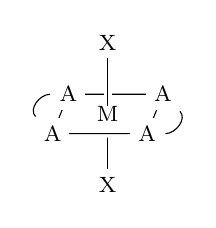
\begin{tikzpicture}[
                    every node/.append style={black,fill=white}
                ]
                    \footnotesize
                    \node (M) {M};
                    \draw (M) -- ++(0,-0.9) node(X2){\ce{X}};
                    \draw [white,very thick,double=black,double distance=0.4pt]
                        (-0.7,-0.25) node(A1){\ce{A}}
                        -- (0.5,-0.25) node(A2){\ce{A}}
                        -- (0.7,0.25) node(A3){\ce{A}}
                        -- (-0.5,0.25) node(A4){\ce{A}}
                        -- cycle
                    ;
                    \draw [white,very thick,double=black,double distance=0.4pt] ([yshift=-1mm]M.north) -- (M) -- ++(0,0.9) node(X1){\ce{X}};

                    \draw (A1) to[out=135,in=180] (A4);
                    \draw (A2) to[out=0,in=-45] (A3);
                \end{tikzpicture}
                \caption{\emph{trans} is achiral.}
                \label{fig:octahedralChiralityTwoa}
            \end{subfigure}
            \begin{subfigure}[b]{0.25\linewidth}
                \centering
                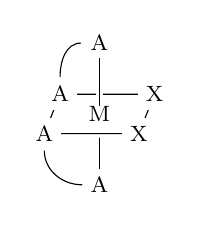
\begin{tikzpicture}[
                    every node/.append style={black,fill=white}
                ]
                    \footnotesize
                    \node (M) {M};
                    \draw (M) -- ++(0,-0.9) node(X2){\ce{A}};
                    \draw [white,very thick,double=black,double distance=0.4pt]
                        (-0.7,-0.25) node(A1){\ce{A}}
                        -- (0.5,-0.25) node(A2){\ce{X}}
                        -- (0.7,0.25) node(A3){\ce{X}}
                        -- (-0.5,0.25) node(A4){\ce{A}}
                        -- cycle
                    ;
                    \draw [white,very thick,double=black,double distance=0.4pt] ([yshift=-1mm]M.north) -- (M) -- ++(0,0.9) node(X1){\ce{A}};

                    \draw (X1) to[out=180,in=90] (A4);
                    \draw (A1) to[out=-90,in=180] (X2);
                \end{tikzpicture}
                \caption{Left-handed screw.}
                \label{fig:octahedralChiralityTwob}
            \end{subfigure}
            \begin{subfigure}[b]{0.25\linewidth}
                \centering
                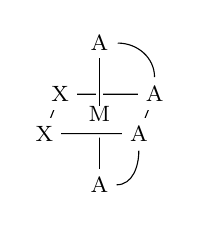
\begin{tikzpicture}[
                    every node/.append style={black,fill=white}
                ]
                    \footnotesize
                    \node (M) {M};
                    \draw (M) -- ++(0,-0.9) node(X2){\ce{A}};
                    \draw [white,very thick,double=black,double distance=0.4pt]
                        (-0.7,-0.25) node(A1){\ce{X}}
                        -- (0.5,-0.25) node(A2){\ce{A}}
                        -- (0.7,0.25) node(A3){\ce{A}}
                        -- (-0.5,0.25) node(A4){\ce{X}}
                        -- cycle
                    ;
                    \draw [white,very thick,double=black,double distance=0.4pt] ([yshift=-1mm]M.north) -- (M) -- ++(0,0.9) node(X1){\ce{A}};

                    \draw (X1) to[out=0,in=90] (A3);
                    \draw (A2) to[out=-90,in=0] (X2);
                \end{tikzpicture}
                \caption{Right-handed screw.}
                \label{fig:octahedralChiralityTwoc}
            \end{subfigure}
            \caption{Chirality of octahedral complexes with two bidentate ligands.}
            \label{fig:octahedralChiralityTwo}
        \end{figure}
        \begin{itemize}
            \item As we can see in Figure \ref{fig:octahedralChiralityTwo}, \emph{trans}-\ce{M(A-A)2X2} is not chiral, but \emph{cis}-\ce{M(A-A)2X2} is chiral with two specially named forms.
        \end{itemize}
        \item Octahedral complexes with three bidentate ligands:
        \begin{itemize}
            \item \emph{Also known as} \textbf{propellor chirality}.
            \item Left-handed helices are $\Lambda$ form, while right-handed helices are $\Delta$ form.
        \end{itemize}
    \end{itemize}
\end{itemize}



\section{Module 31: Crystal Field Theory}
\begin{itemize}
    \item The first attempt to understand and rationalize the electronic structure of transition metal complexes.
    \begin{itemize}
        \item Originally introduced to analyze crystals' electronic structure.
        \item Since the coordination of a central atom in a crystalline closely mimics that of it in a coordination complex, the concepts of crystal field theory can easily be transferred to chemistry.
    \end{itemize}
    \item Suggested reading: \textcite{bib:MiesslerFischerTarr} Section 10.2.
    \item Refresher on $d$-orbitals.
    \begin{itemize}
        \item There are four $d$-orbitals with four lobes and one strange $d_{z^2}$ orbital.
        \item Higher energy level ones have lobes corresponding to the change in sign of the radial component..
        \item The $d_{z^2}$ orbital is a linear combination of two four-lobed orbitals; it is created to reconcile mathematical theory with physical reality (the Pauli exclusion principle).
    \end{itemize}
    \item Crystal field theory describes an electrostatic (ionic) approach to bonding --- it is so named because it was first applied to crystalline substances.
    \begin{itemize}
        \item Interactions between filled $d$-orbitals and ligands with excessive electrons are repulsive.
    \end{itemize}
    \item Assumptions:
    \begin{enumerate}
        \item Metal ion at the center.
        \item Ligands are treated as point charges.
        \item Bonding occurs through \ce{M+} and \ce{L-} electrostatic attraction.
        \item Bonding is purely ionic.
        \item \ce{M} and \ce{L} electrons repel each other.
        \item $d$-orbital degeneracy is broken as ligands approach.
    \end{enumerate}
    \item Consider $d$-orbitals bonding to six ligands.
    \begin{itemize}
        \item Keep Coulomb's Law ($E\propto\frac{q_1q_2}{r}$) in mind: $d$-orbitals that overlap more with the ligands (smaller $r$) will be more destabilized (higher $E$).
        \item $d_{z^2}$ overlaps with the two axial ligands, and $d_{x^2-y^2}$ overlaps with the four equatorial ligands.
        \item None of $d_{xy}$, $d_{xz}$, and $d_{yz}$ overlap significantly with any ligands.
        \item Therefore, the five degenerate $d$-orbitals split into the \textbf{$\bm{t_{2g}}$ set} and the \textbf{$\bm{e_g}$ set}.
        \item When the orbitals split, they maintain an energetic "center of mass," i.e., their combined energy as molecular orbitals must still be equal to their combined energy as degenerate, atomic orbitals. Thus, the stabilization energy of the three orbitals in the $t_{2g}$ set is $-\frac{2}{5}\Delta$ while the destabilization energy of the two orbbitals in the $e_g$ set is $\frac{3}{5}\Delta$, where $\Delta$ is the \textbf{crystal field splitting parameter}.
    \end{itemize}
    \item \textbf{$\bm{t_{2g}}$ set}: The three orbitals that lie between the ligand donor atoms.
    \item \textbf{$\bm{e_g}$ set}: The two orbitals that lie along the Cartesian coordinates, and so are adjacent to the donor atoms of the ligands, raising the set in energy.
    \item \textbf{Crystal field splitting parameter}: Different ligands produce different extents of splitting between the $e_g$ and the $t_{2g}$ levels. This energy difference is the crystal field splitting parameter. \emph{Units} $\si{\per\centi\meter}$. \emph{Also known as} $\bm{\Delta}$, $\bm{10Dq}$.
    \item Experimental verification of orbital splitting.
    \begin{itemize}
        \item Consider a coordination complex with just one $d$-electron, i.e., electron configuration $d^1$.
        \begin{itemize}
            \item An example is \ce{[Ti(H2O)6]^3+}.
        \end{itemize}
        \item In such a complex, the electron will occupy the lowest energy orbital available, i.e., one of the three degenerate $t_{2g}$ orbitals.
        \item Shining light on the complex can promote the $t_{2g}$ electron into the $e_g$ energy level.
        \item The UV-Vis absorption spectrum reveals that this transition occurs with a maximum at $\SI{20300}{\per\centi\meter}$, or $\Delta=\SI[per-mode=symbol]{243}{\kilo\joule\per\mole}\neq 0$.
    \end{itemize}
    \item Note that $\SI{1000}{\per\centi\metre}=\SI[per-mode=symbol]{11.96}{\kilo\joule\per\mole}=\SI[per-mode=symbol]{2.86}{kcal\per\mole}=\SI{0.124}{eV}$.
    \item \textbf{Crystal field stabilization energy}: The overall change in energy when the $d$-subshell splits, which is given by $(0.4n(t_{2g})-0.6n(e_g))\Delta$ where $n(t_{2g})$ and $n(e_g)$ are the numbers of electrons in the $t_{2g}$ and $e_g$ levels respectively. \emph{Also known as} \textbf{CFSE}.
    \begin{itemize}
        \item When splitting of the $d$-subshell occurs, the occupation of the lower energy $t_{2g}$ level by electrons causes a stabilization of the complex, whereas occupation of the $e_g$ level causes a rise in energy. The $t_{2g}$ level drops by $0.4\Delta$, whereas the $e_g$ level is raised by $0.6\Delta$.
    \end{itemize}
    \item High and low-spin complexes:
    \begin{itemize}
        \item Whether a complex is \textbf{high-spin} or \textbf{low-spin} depends on $\Delta$.
        \item If $\Delta>P$ where $P$ is the \textbf{spin-pairing energy}, then the complex is low-spin, and vice versa if $\Delta<P$.
    \end{itemize}
    \item \textbf{High-spin} (complex): A complex with $d^4$ to $d^8$ electron configuration, where the electrons spread out and occupy the whole $d$-subshell.
    \begin{itemize}
        \item High-spin complexes are often paramagnetic.
        \item Electrons fill the whole $d$-subshell according to Hund's rule.
    \end{itemize}
    \item \textbf{Low-spin} (complex): A complex with $d^4$ to $d^8$ electron configurations, where the $t_{2g}$ energy level is filled first.
    \begin{itemize}
        \item Low-spin complexes are often diamagnetic.
    \end{itemize}
    \item \textbf{Spin-pairing energy}: The energy required to take pairs of electrons with the same spin orientation, and pair them up with the opposite spin. \emph{Also known as} $\bm{P}$.
    \item Calculating CFSE of $d^0$ to $d^{10}$ high-spin \ce{M} (II) ions.
    \begin{figure}[H]
        \centering
        \pgfdeclareplotmark{elip}{\pgfpathellipse{\pgfpoint{0pt}{0pt}}{\pgfpoint{4pt}{0pt}}{\pgfpoint{0pt}{1pt}}\pgfusepathqfill}
        \begin{tikzpicture}[xscale=0.5,yscale=2]
            \footnotesize
            \draw (11,0) -- node[below=5mm]{\small Number of $d$-electrons} (0,0) -- node[rotate=90,left=1cm,anchor=center]{CFSE (multiples of $\Delta$)} (0,1.4);
            \node [below left=1mm] {$0$};
            \foreach \x in {1,...,10} {
                \draw (\x,0.05) -- ++(0,-0.1) node[below]{$\x$};
            }
            \foreach \y in {0.2,0.4,0.6,0.8,1,1.2,1.4} {
                \draw (0.2,\y) -- ++(-0.4,0) node[left]{$\y$};
            }

            \draw [grx,thick] plot [mark=elip] coordinates {(0,0) (1,0.4) (2,0.8) (3,1.2) (4,0.6) (5,0) (6,0.4) (7,0.8) (8,1.2) (9,0.6) (10,0)};
        \end{tikzpicture}
        \caption{CFSE as a function of the number of $d$-electrons.}
        \label{fig:CFSEcurve}
    \end{figure}
    \begin{itemize}
        \item Most first row and many second and third row transition elements will be prone to forming high-spin complexes.
        \item The variation shown in Figure \ref{fig:CFSEcurve} reveals that complexes of metal ions with high CFSE (such as \ce{Ni} (II)) will undergo greater stabilization, and vice versa for metal ions with low CFSE (such as \ce{Ca} (II)).
        \item The predicted variation matches relatively well with formation constant values ($\log K_1$) obtained experimentally for these compounds.
    \end{itemize}
    \item We can also look at orbital splitting in coordination compounds of other geometries.
    \begin{itemize}
        \item In $T_d$ compounds, for example, the splitting is flipped with the $d_{xy,xz,yz}$ orbitals destabilized and the $d_{x^2-y^2,z^2}$ orbitals stabilized.
        \item We can also look analyze linear and square planar geometries.
    \end{itemize}
    \item Merits of crystal field theory:
    \begin{itemize}
        \item Can be used to predict the most favorable geometry for the complex.
        \item Can account for why some complexes are tetrahedral and others are square planar.
        \item Useful in interpreting magnetic properties.
        \item The colors of many transition metal complexes can be rationalized.
    \end{itemize}
    \item Limitations of crystal field theory:
    \begin{itemize}
        \item Becomes less accurate as delocalization (covalent character) increases.
        \item Point charge does not accurately represent complexes.
        \item Does not account for $\pi$ bonding interactions.
        \item Does not account for the relative strengths of the ligands.
    \end{itemize}
\end{itemize}



\section[Module 32: Ligand Field Theory for the \texorpdfstring{$O_h$}{TEXT} \texorpdfstring{$\sigma$}{TEXT}-Only Case]{Module 32: Ligand Field Theory for the \texorpdfstring{$\bm{O_h}$}{TEXT} \texorpdfstring{$\bm{\sigma}$}{TEXT}-Only Case}
\begin{itemize}
    \item \marginnote{2/17:}Suggested reading: \textcite{bib:MiesslerFischerTarr} Section 10.3.
    \item Ligand field theory:
    \begin{itemize}
        \item Application of molecular orbital theory to transition metal complexes.
        \item Ligands are not point charges.
        \item Takes into account $\pi$ bonding.
        \begin{itemize}
            \item I.e., accounts for the fact that ligands can be $\sigma$-donors, $\pi$-donors, $\pi$-acceptors, or sometimes multiple simultaneously.
        \end{itemize}
        \item Can be used to explain spectrochemical series.
        \item Better than valence-bond model or crystal field theory at explaining experimental data.
    \end{itemize}
    \item Octahedral $\sigma$-only MO diagram workflow:
    \begin{enumerate}
        \item Assign a point group.
        \item Choose basis function.
        \item Apply operations.
        \item Generate a reducible representation.
        \item Reduce to irreducible representations.
        \item Combine orbitals by their symmetry.
        \item Fill MOs with $\e[-]$.
        \item Generate SALCs of peripheral atoms.
        \item Draw peripheral atom SALC with central atom orbital to generate bonding/antibonding MOs.
    \end{enumerate}
    \item \ce{MH6} example.
    \begin{itemize}
        \item Point group: $O_h$.
        \item Basis funtions: $1s$-orbitals on the ligands (you can also choose the $\sigma$-bond vectors if you wish [if it's easier for you]), and $s,p,d$-orbitals on the metal center.
        \item Apply operations \& generate a reducible representation.
        \begin{align*}
            \Gamma_{\ce{H}} &= (6,0,0,2,2,0,0,0,4,2) = A_{1g}+T_{1u}+E_g\\
            \Gamma_{\ce{M}_{s}} &= A_{1g}\\
            \Gamma_{\ce{M}_{p}} &= T_{1u}\\
            \Gamma_{\ce{M}_{d_{x^2-y^2,z^2}}} &= E_g\\
            \Gamma_{\ce{M}_{d_{xy,xz,yz}}} &= T_{2g}
        \end{align*}
        \item Combine orbitals by their symmetry.
        \begin{figure}[h!]
            \centering
            \begin{tikzpicture}[
                yscale=0.15,
                every node/.prefix style={black}
            ]
                \footnotesize
                \path (-7,-20) -- (7,-20);
        
                \draw [ultra thick,gry]
                    (-4.7,-10) -- node[below]{$T_{1u}$} ++(0.5,0) ++(0.1,0) -- node[below]{$T_{1u}$} ++(0.5,0) ++(0.1,0) -- node[below]{$T_{1u}$} ++(0.5,0) coordinate (4p)
                    (-3.5,-21) -- node[below]{$A_{1g}$} ++(0.5,0) coordinate (4s)
                    (-5.9,-30) -- node[below]{$E_g$} ++(0.5,0) ++(0.1,0) -- node[below]{$E_g$} ++(0.5,0) coordinate (3d2) ++(0.1,0) -- node[below]{$T_{2g}$} ++(0.5,0) ++(0.1,0) -- node[below]{$T_{2g}$} ++(0.5,0) ++(0.1,0) -- node[below]{$T_{2g}$} ++(0.5,0) coordinate (3d1)
                    (3,-36) coordinate (1s1) -- node[below]{$T_{1u}$} ++(0.5,0) ++(0.1,0) -- node[below]{$T_{1u}$} ++(0.5,0) ++(0.1,0) -- node[below]{$T_{1u}$} ++(0.5,0) ++(0.1,0) coordinate (1s2) -- node[below]{$E_g$} ++(0.5,0) ++(0.1,0) -- node[below]{$E_g$} ++(0.5,0) ++(0.1,0) coordinate (1s3) -- node[below]{$A_{1g}$} ++(0.5,0)
                ;
                \draw [ultra thick]
                    (-0.85,-2) coordinate (t1uul) -- ++(0.5,0) ++(0.1,0) -- node[below]{$t_{1u}$} ++(0.5,0) ++(0.1,0) -- ++(0.5,0) coordinate (t1uur)
                    (-0.85,-8) coordinate (a1gul) -- node[below]{$a_{1g}$} ++(1.7,0) coordinate (a1gur)
                    (-0.85,-19) coordinate (egul) -- ++(0.8,0) node[below,xshift=0.05cm]{$e_g$} ++(0.1,0) -- ++(0.8,0) coordinate (egur)
                    (-0.85,-30) coordinate (t2g) -- ++(0.5,0) ++(0.1,0) -- node[below]{$t_{2g}$} ++(0.5,0) ++(0.1,0) -- ++(0.5,0)
                    (-0.85,-37) coordinate (t1ull) -- ++(0.5,0) ++(0.1,0) -- node[below]{$t_{1u}$} ++(0.5,0) ++(0.1,0) -- ++(0.5,0) coordinate (t1ulr)
                    (-0.85,-43) coordinate (egll) -- ++(0.8,0) node[below,xshift=0.05cm]{$e_g$} ++(0.1,0) -- ++(0.8,0) coordinate (eglr)
                    (-0.85,-50) coordinate (a1gll) -- node[below]{$a_{1g}$} ++(1.7,0) coordinate (a1glr)
                ;
        
                \begin{scope}[on background layer]
                    \draw [thick,grx,densely dashed]
                        (4p) -- (t1uul)
                        (4p) -- (t1ull)
                        (4s) -- (a1gul)
                        (4s) -- (a1gll)
                        (3d1) -- (t2g)
                        (3d2) -- (egul)
                        (3d2) -- (egll)
                        (1s1) -- (t1uur)
                        (1s1) -- (t1ulr)
                        (1s2) -- (egur)
                        (1s2) -- (eglr)
                        (1s3) -- (a1gur)
                        (1s3) -- (a1glr)
                    ;
                \end{scope}

                \node at (-4.45,-56) {\small\ce{M}};
                \node at (4.75,-56) {\small$6\times \ce{H}$};
            \end{tikzpicture}
            \caption{\ce{MH6} orbital diagram.}
            \label{fig:orbitalDiagram-MH6}
        \end{figure}
        \begin{itemize}
            \item In a transition metal compound/coordination complex, the $t_{2g}$ MOs would be the HOMOs and the antibonding $e_g$ MOs would be the LUMOs.
            \item Since the $t_{2g}$ orbitals are nonbonding, they are reflective of the energy of the metal $d$-orbitals. Thus, the energy difference between them and the $e_g$ orbitals is equal to the amount by which the $e_g$ orbitals' energy changes during bonding, i.e., the splitting parameter. This energy change is also indicative of the antibonding character of the $e_g$ orbitals, and consequently the strength of the bonding (bigger $\Delta$ implies higher energy $e_g$ orbitals implies stronger bonding).
            \item In LFT, we call this quantity the \textbf{ligand field splitting parameter}, as opposed to the crystal field splitting parameter.
            \item Pauses to consider \textbf{weak field ligands} and \textbf{strong field ligands}.
        \end{itemize}
        \item Generate SALCs of peripheral atoms.
        \begin{align*}
            \Psi(a_{1g}) &= c_1(4s)+c_2(\sigma_1+\sigma_2+\sigma_3+\sigma_4+\sigma_5+\sigma_6)\\
            \Psi_z(t_{1u}) &= c_3(4p_z)+c_4(\sigma_1-\sigma_6)\\
            \Psi_x(t_{1u}) &= c_3(4p_x)+c_4(\sigma_4-\sigma_2)\\
            \Psi_y(t_{1u}) &= c_3(4p_y)+c_4(\sigma_3-\sigma_5)\\
            \Psi_{z^2}(e_g) &= c_5(3d_{z^2})+c_6(\sigma_1+\sigma_6)+c_7(-\sigma_2-\sigma_3-\sigma_4-\sigma_5)\\
            \Psi_{x^2-y^2}(e_g) &= c_8(3d_{x^2-y^2})+c_9(\sigma_2-\sigma_3+\sigma_4-\sigma_5)
        \end{align*}
        \begin{itemize}
            \item Recall that the coefficients reflect the degree of overlap.
            \item Note that for the $\Psi(t_{1u})$ wavefunctions, the in-plane $\sigma$-orbitals have zero overlap with the perpendicular $4p$ orbital, hence their coefficient of 0.
        \end{itemize}
        \item Draw peripheral atom SALC with central atom orbital to generate bonding/antibonding MOs.
        \begin{figure}[h!]
            \centering
            \begin{subfigure}[b]{0.19\linewidth}
                \centering
                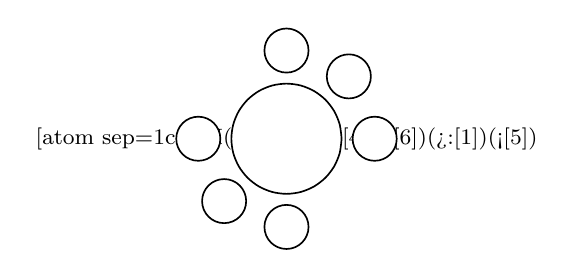
\begin{tikzpicture}[scale=0.7,z={(0.8,0.65)}]
                    \footnotesize
                    \node {\chemfig[atom sep=1cm]{M(-[0])(-[2])(-[4])(-[6])(>:[1])(<[5])}};
                    \filldraw [semithick,fill=white] plot[domain=0:2*pi,smooth,variable=\thta] ({\thta r}:1);
        
                    \filldraw [semithick,fill=white] (0:1.6) circle (4mm);
                    \filldraw [semithick,fill=white] (45:1.6) circle (4mm);
                    \filldraw [semithick,fill=white] (90:1.6) circle (4mm);
                    \filldraw [semithick,fill=white] (180:1.6) circle (4mm);
                    \filldraw [semithick,fill=white] (225:1.6) circle (4mm);
                    \filldraw [semithick,fill=white] (270:1.6) circle (4mm);
                \end{tikzpicture}
                \caption{$\Psi(a_{1g})$.}
                \label{fig:SALCs-MH6a}
            \end{subfigure}\\[1em]
            \begin{subfigure}[b]{0.19\linewidth}
                \centering
                \begin{tikzpicture}[scale=0.7,z={(0.8,0.65)}]
                    \footnotesize
                    \node {\chemfig[atom sep=1cm]{M(-[0])(-[2])(-[4])(-[6])(>:[1])(<[5])}};
                    \filldraw [semithick,fill=grt] (0,{-6^0.5/4},0) circle (6^0.5/4);
                    \filldraw [semithick,fill=white] (0,{6^0.5/4},0) circle (6^0.5/4);
                    \node {\chemfig[atom sep=1cm]{\phantom{M}(-[0,,,,opacity=0])(-[2,,,,opacity=0])(-[4,,,,opacity=0])(-[6,,,,opacity=0])(>:[1,,,,opacity=0])(<[5])}};
        
                    \filldraw [semithick,fill=white] (90:1.6) circle (4mm);
                    \filldraw [semithick,fill=grt] (270:1.6) circle (4mm);
                \end{tikzpicture}
                \caption{$\Psi_z(t_{1u})$.}
                \label{fig:SALCs-MH6b}
            \end{subfigure}
            \begin{subfigure}[b]{0.19\linewidth}
                \centering
                \begin{tikzpicture}[scale=0.7,z={(0.8,0.65)}]
                    \footnotesize
                    \node {\chemfig[atom sep=1cm]{M(-[0])(-[2])(-[4])(-[6])(>:[1])(<[5])}};
                    \filldraw [semithick,fill=grt] ({-6^0.5/4},0,0) circle (6^0.5/4);
                    \filldraw [semithick,fill=white] ({6^0.5/4},0,0) circle (6^0.5/4);
                    \node {\chemfig[atom sep=1cm]{\phantom{M}(-[0,,,,opacity=0])(-[2,,,,opacity=0])(-[4,,,,opacity=0])(-[6,,,,opacity=0])(>:[1,,,,opacity=0])(<[5])}};
        
                    \filldraw [semithick,fill=white] (0:1.6) circle (4mm);
                    \filldraw [semithick,fill=grt] (180:1.6) circle (4mm);
                \end{tikzpicture}
                \caption{$\Psi_x(t_{1u})$.}
                \label{fig:SALCs-MH6c}
            \end{subfigure}
            \begin{subfigure}[b]{0.19\linewidth}
                \centering
                \begin{tikzpicture}[scale=0.7,z={(0.8,0.65)}]
                    \footnotesize
                    \node {\chemfig[atom sep=1cm]{M(-[0])(-[2])(-[4])(-[6])(>:[1])(<[5])}};
                    \filldraw [semithick,fill=white] (0,0,{6^0.5/4}) circle (6^0.5/4);
                    \filldraw [semithick,fill=grt] (0,0,{-6^0.5/4}) circle (6^0.5/4);
                    \node {\chemfig[atom sep=1cm]{\phantom{M}(-[0])(-[2])(-[4,,,,opacity=0])(-[6,,,,opacity=0])(>:[1,,,,opacity=0])(<[5,,,,opacity=0])}};
        
                    \filldraw [semithick,fill=white] (45:1.6) circle (4mm);
                    \filldraw [semithick,fill=grt] (225:1.6) circle (4mm);
                \end{tikzpicture}
                \caption{$\Psi_y(t_{1u})$.}
                \label{fig:SALCs-MH6d}
            \end{subfigure}\\[1em]
            \begin{subfigure}[b]{0.19\linewidth}
                \centering
                \begin{tikzpicture}[scale=0.7,z={(0.8,0.65)}]
                    \footnotesize
                    \node {\chemfig[atom sep=1cm]{M(-[0])(-[2])(-[4])(-[6])(>:[1])(<[5])}};
                    \filldraw [semithick,fill=white] plot [domain=0.63:2.51,smooth,variable=\thta] ({\thta r}:{0.5*2.5^0.5*(3*sin(\thta r)^2-1)});
                    \filldraw [semithick,fill=white] plot [domain=3.75:5.67,smooth,variable=\thta] ({\thta r}:{0.5*2.5^0.5*(3*sin(\thta r)^2-1)});
                    \filldraw [semithick,fill=grt] (-0.4,0,0) arc[start angle=120,end angle=60,x radius=0.8cm,y radius=0.9cm] arc[start angle=-60,end angle=-120,x radius=0.8cm,y radius=0.9cm];
                    \filldraw [semithick,fill=white] ({0.73 r}:{0.5*2.5^0.5*(3*sin(0.73 r)^2-1)}) to[out=-125,in=-55] ({2.41 r}:{0.5*2.5^0.5*(3*sin(2.41 r)^2-1)});
        
                    \filldraw [semithick,fill=grt] (0:1.6) circle (4mm);
                    \filldraw [semithick,fill=grt] (45:1.6) circle (4mm);
                    \filldraw [semithick,fill=white] (90:1.6) circle (4mm);
                    \filldraw [semithick,fill=grt] (180:1.6) circle (4mm);
                    \filldraw [semithick,fill=grt] (225:1.6) circle (4mm);
                    \filldraw [semithick,fill=white] (270:1.6) circle (4mm);
                \end{tikzpicture}
                \caption{$\Psi_{z^2}(e_g)$.}
                \label{fig:SALCs-MH6e}
            \end{subfigure}
            \begin{subfigure}[b]{0.19\linewidth}
                \centering
                \begin{tikzpicture}[scale=0.7,z={(0.8,0.65)}]
                    \footnotesize
                    \node {\chemfig[atom sep=1cm]{M(-[0])(-[2])(-[4])(-[6])(>:[1])(<[5])}};
                    \filldraw [semithick,fill=grt,scale=1.3,rotate=40] plot [domain=-pi/2:pi/2,smooth,variable=\thta] ({\thta r}:{15^0.5/4*cos(\thta r)^2});
                    \filldraw [semithick,fill=white,scale=1.5] plot [domain=pi/2:3*pi/2,smooth,variable=\thta] ({\thta r}:{15^0.5/4*cos(\thta r)^2});
                    \filldraw [semithick,fill=white,scale=1.5] plot [domain=-pi/2:pi/2,smooth,variable=\thta] ({\thta r}:{15^0.5/4*cos(\thta r)^2});
                    \filldraw [semithick,fill=grt,scale=1.3,rotate=40] plot [domain=pi/2:3*pi/2,smooth,variable=\thta] ({\thta r}:{15^0.5/4*cos(\thta r)^2});
                    \node {\chemfig[atom sep=1cm]{\phantom{M}(-[0,,,,opacity=0])(-[2])(-[4,,,,opacity=0])(-[6,,,,opacity=0])(>:[1,,,,opacity=0])(<[5,,,,opacity=0])}};
        
                    \filldraw [semithick,fill=white] (0:1.6) circle (4mm);
                    \filldraw [semithick,fill=grt] (45:1.6) circle (4mm);
                    \filldraw [semithick,fill=white] (180:1.6) circle (4mm);
                    \filldraw [semithick,fill=grt] (225:1.6) circle (4mm);
                \end{tikzpicture}
                \caption{$\Psi_{x^2-y^2}(e_g)$.}
                \label{fig:SALCs-MH6f}
            \end{subfigure}
            \caption{\ce{MH6} bonding and antibonding MOs.}
            \label{fig:SALCs-MH6}
        \end{figure}
    \end{itemize}
    \item \textbf{Weak field ligand}: A ligand with high electronegativity, and thus low energy frontier orbitals.
    \begin{itemize}
        \item Weak $\sigma$ donor.
        \item Weak Lewis base.
        \item Weaker bonding interaction.
        \item Smaller $\Delta_o$.
    \end{itemize}
    \item \textbf{Strong field ligand}: A ligand with comparable energy frontier orbitals to the $d$-orbitals of the metal cation.
    \begin{itemize}
        \item Strong $\sigma$ donor.
        \item Strong Lewis base.
        \item Stronger bonding interaction.
        \item Larger $\Delta_o$.
    \end{itemize}
    \item Size matters more than Lewis basicity:
    \begin{itemize}
        \item Stronger Lewis base $\Rightarrow$ larger $\Delta_o$.
        \item Smaller ligand $\Rightarrow$ larger $\Delta_o$.
        \item However, size overall is more important.
        \begin{itemize}
            \item This is related to hardness and softness --- with a hard Lewis acid metal center, harder ligands will bond with greater strengths.
        \end{itemize}
    \end{itemize}
    \item For the halides' $\Delta_o$: $\ce{I-}<\ce{Br-}<\ce{Cl-}<\ce{F-}$.
    \item If we use $p$-orbitals pointing toward the center as bases for our peripheral atoms instead of $s$-orbitals, we get the exact same result.
    \item Factors that influence $\Delta_\text{oct}=\Delta_o=10Dq$.
    \begin{itemize}
        \item Metal oxidation state: Increasing the charge increases $\Delta$.
        \item Principal quantum number: Increasing $n$ (going down a period on the periodic table) increases $\Delta$, too.
        \item Nature of the ligand:
        \begin{table}[h!]
            \centering
            \small
            \renewcommand{\arraystretch}{1.4}
            \begin{tabular}{|c|c|c|c|}
                \hline
                \textbf{\ce{L}} & \textbf{Ligand Type} & $\bm{z}$ & $\bm{\Delta_o\ (\textbf{cm}^{-1})}$\\
                \hline
                \ce{Cl-} & $\sigma,\pi$-donor & $3-$ & $\num{13700}$\\
                \ce{H2O} & $\sigma$-donor & $3+$ & $\num{17400}$\\
                \ce{NH3} & $\sigma$-donor & $3+$ & $\num{21500}$\\
                \ce{CN-} & $\sigma$-donor/$\pi$-acceptor & $3-$ & $\num{26600}$\\
                \hline
            \end{tabular}
            \caption{How the nature of the ligand influences $\Delta$.}
            \label{tab:natureOfTheLigand}
        \end{table}
    \end{itemize}
\end{itemize}



\section[Module 33: Ligand Field Theory for the \texorpdfstring{$O_h$}{TEXT} \texorpdfstring{$\sigma+\pi$}{TEXT} Case]{Module 33: Ligand Field Theory for the \texorpdfstring{$\bm{O_h}$}{TEXT} \texorpdfstring{$\bm{\sigma+\pi}$}{TEXT} Case}
\begin{itemize}
    \item Consider cyano-ligands (isoelectronic to \ce{CO} and \ce{NO+}).
    \begin{itemize}
        \item HOMO is perfect for $\sigma$ bonding via donation.
        \item LUMO is perfect for $\pi$ acceptance from metal $d$-orbitals.
        \begin{figure}[h!]
            \centering
            \begin{tikzpicture}
                \footnotesize
                \node {\ce{M}};
                \node at (2,0) {\ce{C}};
                \node at (3,0) {\ce{N}};
        
                \filldraw [semithick,fill=grt,rotate=45] (0.7,0) ellipse (4mm and 2.5mm);
                \filldraw [semithick,fill=white,rotate=135] (0.7,0) ellipse (4mm and 2.5mm);
                \filldraw [semithick,fill=grt,rotate=225] (0.7,0) ellipse (4mm and 2.5mm);
                \filldraw [semithick,fill=white,rotate=315] (0.7,0) ellipse (4mm and 2.5mm);
        
                \filldraw [semithick,fill=grt] (2,0.6) ellipse (6mm and 3.5mm);
                \filldraw [semithick,fill=white] (2,-0.6) ellipse (6mm and 3.5mm);
                \filldraw [semithick,fill=white] (3,0.5) ellipse (3mm and 2mm);
                \filldraw [semithick,fill=grt] (3,-0.5) ellipse (3mm and 2mm);
        
                \draw [semithick,-stealth] (0.6,0.6) to[out=30,in=135] (1.8,0.5);
                \draw [semithick,-stealth] (0.6,-0.6) to[out=-30,in=-135] (1.8,-0.5);
            \end{tikzpicture}
            \caption{LUMO $\pi$-acceptance.}
            \label{fig:piAcceptance}
        \end{figure}
        \begin{itemize}
            \item $d_{xz}$ and $\pi^*$ orbitals combine with stabilization energy $e_\pi$.
        \end{itemize}
        \item This is how we determine what kinds of donors the ligands in Table \ref{tab:natureOfTheLigand} are. For \ce{H2O}, for example, it is not a $\pi$-acceptor because its LUMO is a $\sigma^*$ orbital, not a $\pi^*$ one (see Figure \ref{fig:orbitalDiagram-H2O}).
    \end{itemize}
    \item Octahedral $\sigma+\pi$ bonding:
    \begin{figure}[H]
        \centering
        \begin{tikzpicture}[
            scale=0.8,
            every node/.append style={black}
        ]
            \footnotesize
            \draw [->] (-4,0,0) -- (4,0,0) node[right]{\small$Y$};
            \draw [->] (0,-4,0) -- (0,4,0) node[above]{\small$Z$};
            \draw [->] (0,0,-4) -- (0,0,4) node[below left]{\small$X$};
    
            \draw [grx,thick,-stealth] (3.7,0,0) -- (2.7,0,0) node[above left=-1mm]{$y$};
            \draw [grx,thick,-stealth] (3.7,0,0) -- (3.7,1,0) node[above]{$x$};
            \draw [grx,thick,-stealth] (3.7,0,0) -- (3.7,0,1) node[below left=-1mm]{$z$};
    
            \draw [grx,thick,-stealth] (0,0,-3.7) -- (0,0,-2.7) node[above left=-1mm]{$y$};
            \draw [grx,thick,-stealth] (0,0,-3.7) -- (0,-1,-3.7) node[below]{$x$};
            \draw [grx,thick,-stealth] (0,0,-3.7) -- (-1,0,-3.7) node[left]{$z$};
    
            \draw [grx,thick,-stealth] (-3.7,0,0) -- (-2.7,0,0) node[above right=-1mm]{$y$};
            \draw [grx,thick,-stealth] (-3.7,0,0) -- (-3.7,0,-1) node[above right=-1mm]{$x$};
            \draw [grx,thick,-stealth] (-3.7,0,0) -- (-3.7,-1,0) node[below]{$z$};
    
            \draw [grx,thick,-stealth] (0,0,3.7) -- (0,0,2.7) node[above left=-1mm]{$y$};
            \draw [grx,thick,-stealth] (0,0,3.7) -- (1,0,3.7) node[right]{$x$};
            \draw [grx,thick,-stealth] (0,0,3.7) -- (0,1,3.7) node[above]{$z$};
    
            \draw [grx,thick,-stealth] (0,3.7,0) -- (0,2.7,0) node[below right=-1mm]{$y$};
            \draw [grx,thick,-stealth] (0,3.7,0) -- (0,3.7,1) node[below left=-1mm]{$x$};
            \draw [grx,thick,-stealth] (0,3.7,0) -- (1,3.7,0) node[right]{$z$};
    
            \draw [grx,thick,-stealth] (0,-3.7,0) -- (0,-2.7,0) node[above left=-1mm]{$y$};
            \draw [grx,thick,-stealth] (0,-3.7,0) -- (-1,-3.7,0) node[left]{$x$};
            \draw [grx,thick,-stealth] (0,-3.7,0) -- (0,-3.7,-1) node[above right=-1mm]{$z$};
        \end{tikzpicture}
        \caption{Octahedral $\pi$-ligand coordinate systems.}
        \label{fig:piOctahedralLigand}
    \end{figure}
    \begin{itemize}
        \item Generate a reducible representation: $\Gamma_{L\pi_{x,z}}=(12,0,0,-4,0,0,0,0,0)=T_{1g}+T_{2g}+T_{1u}+T_{2u}$.
        \item Combine orbitals by their symmetry.
        \begin{figure}[H]
            \centering
            \begin{tikzpicture}[
                yscale=0.25,
                every node/.prefix style={black}
            ]
                \footnotesize
                \path (-7,-20) -- (7,-20);
        
                \draw [ultra thick,gry]
                    (-4.7,-10) -- node[below]{$T_{1u}$} ++(0.5,0) ++(0.1,0) -- node[below]{$T_{1u}$} ++(0.5,0) ++(0.1,0) -- node[below]{$T_{1u}$} ++(0.5,0) coordinate (4p)
                    (-3.5,-21) -- node[below]{$A_{1g}$} ++(0.5,0) coordinate (4s)
                    (-5.9,-30) -- node[below]{$E_g$} ++(0.5,0) ++(0.1,0) -- node[below]{$E_g$} ++(0.5,0) coordinate (3d2) ++(0.1,0) -- node[below]{$T_{2g}$} ++(0.5,0) ++(0.1,0) -- node[below]{$T_{2g}$} ++(0.5,0) ++(0.1,0) -- node[below]{$T_{2g}$} ++(0.5,0) coordinate (3d1)
                    (3,-6) coordinate (2p1) -- node[below]{$T_{1g}$} ++(0.5,0) ++(0.1,0) -- node[below]{$T_{1g}$} ++(0.5,0) ++(0.1,0) -- node[below]{$T_{1g}$} ++(0.5,0) ++(0.1,0) coordinate (2p2) -- node[below]{$T_{2g}$} ++(0.5,0) ++(0.1,0) -- node[below]{$T_{2g}$} ++(0.5,0) ++(0.1,0) -- node[below]{$T_{2g}$} ++(0.5,0) ++(0.1,0) coordinate (2p3) -- node[below]{$T_{1u}$} ++(0.5,0) ++(0.1,0) -- node[below]{$T_{1u}$} ++(0.5,0) ++(0.1,0) -- node[below]{$T_{1u}$} ++(0.5,0) ++(0.1,0) coordinate (2p4) -- node[below]{$T_{2u}$} ++(0.5,0) ++(0.1,0) -- node[below]{$T_{2u}$} ++(0.5,0) ++(0.1,0) -- node[below]{$T_{2u}$} ++(0.5,0)
                    (3,-36) coordinate (1s1) -- node[below]{$T_{1u}$} ++(0.5,0) ++(0.1,0) -- node[below]{$T_{1u}$} ++(0.5,0) ++(0.1,0) -- node[below]{$T_{1u}$} ++(0.5,0) ++(0.1,0) coordinate (1s2) -- node[below]{$E_g$} ++(0.5,0) ++(0.1,0) -- node[below]{$E_g$} ++(0.5,0) ++(0.1,0) coordinate (1s3) -- node[below]{$A_{1g}$} ++(0.5,0)
                ;
                \draw [ultra thick]
                    (-0.85,-1) coordinate (t1uul) -- ++(0.5,0) ++(0.1,0) -- node[below]{$t_{1u}$} ++(0.5,0) ++(0.1,0) -- ++(0.5,0) coordinate (t1uur)
                    (-0.85,-3.5) coordinate (t2gul) -- ++(0.5,0) ++(0.1,0) -- node[below]{$t_{2g}$} ++(0.5,0) ++(0.1,0) -- ++(0.5,0) coordinate (t2gur)
                    (-2,-6) -- ++(0.5,0) ++(0.1,0) -- node[below]{$t_{2u}$} ++(0.5,0) ++(0.1,0) -- ++(0.5,0) ++(0.6,0) -- ++(0.5,0) ++(0.1,0) -- node[below]{$t_{1g}$} ++(0.5,0) ++(0.1,0) -- ++(0.5,0) coordinate (t1g)
                    (-0.85,-9) coordinate (t1uml) -- ++(0.5,0) ++(0.1,0) -- node[below]{$t_{1u}$} ++(0.5,0) ++(0.1,0) -- ++(0.5,0) coordinate (t1umr)
                    (-0.85,-14) coordinate (a1gul) -- node[below]{$a_{1g}$} ++(1.7,0) coordinate (a1gur)
                    (-0.85,-19) coordinate (egul) -- ++(0.8,0) node[below,xshift=0.05cm]{$e_g$} ++(0.1,0) -- ++(0.8,0) coordinate (egur)
                    (-0.85,-32) coordinate (t2gll) -- ++(0.5,0) ++(0.1,0) -- node[below]{$t_{2g}$} ++(0.5,0) ++(0.1,0) -- ++(0.5,0) coordinate (t2glr)
                    (-0.85,-37) coordinate (t1ull) -- ++(0.5,0) ++(0.1,0) -- node[below]{$t_{1u}$} ++(0.5,0) ++(0.1,0) -- ++(0.5,0) coordinate (t1ulr)
                    (-0.85,-41) coordinate (egll) -- ++(0.8,0) node[below,xshift=0.05cm]{$e_g$} ++(0.1,0) -- ++(0.8,0) coordinate (eglr)
                    (-0.85,-45) coordinate (a1gll) -- node[below]{$a_{1g}$} ++(1.7,0) coordinate (a1glr)
                ;
        
                \begin{scope}[on background layer]
                    \draw [thick,grx,densely dashed]
                        (4p) -- (t1uul)
                        (4p) -- (t1uml)
                        (4p) -- (t1ull)
                        (4s) -- (a1gul)
                        (4s) -- (a1gll)
                        (3d1) -- (t2gul)
                        (3d1) -- (t2gll)
                        (3d2) -- (egul)
                        (3d2) -- (egll)
                        (2p1) -- (t1g)
                        (2p2) -- (t2gur)
                        (2p2) -- (t2glr)
                        (2p3) -- (t1uur)
                        (2p3) -- (t1umr)
                        (2p3) -- (t1ulr)
                        (1s1) -- (t1uur)
                        (1s1) -- (t1umr)
                        (1s1) -- (t1ulr)
                        (1s2) -- (egur)
                        (1s2) -- (eglr)
                        (1s3) -- (a1gur)
                        (1s3) -- (a1glr)
                    ;
                \end{scope}
        
                \node at (-4.45,-47) {\small\ce{M}};
                \node at (4.75,-47) {\small$6\times \ce{L}$};
            \end{tikzpicture}
            \caption{\ce{ML6} orbital diagram.}
            \label{fig:orbitalDiagram-ML6}
        \end{figure}
    \end{itemize}
    \begin{figure}[h!]\marginnote{2/22:}
        \centering
        \begin{subfigure}[b]{0.24\linewidth}
            \centering
            \begin{tikzpicture}[scale=0.7,z={(0.8,0.65)}]
                \footnotesize
                \filldraw [semithick,fill=white,yshift=4mm] (45:1.6) circle (4mm);
                \filldraw [semithick,fill=grt,yshift=-4mm] (45:1.6) circle (4mm);
    
                \node {\chemfig[atom sep=1cm]{M(-[0])(-[2])(-[4])(-[6])(>:[1])(<[5])}};
                \filldraw [semithick,fill=grt] (0,{-6^0.5/4},0) circle (6^0.5/4);
                \filldraw [semithick,fill=white] (0,{6^0.5/4},0) circle (6^0.5/4);
                \node {\chemfig[atom sep=1cm]{\phantom{M}(-[0,,,,opacity=0])(-[2,,,,opacity=0])(-[4,,,,opacity=0])(-[6,,,,opacity=0])(>:[1,,,,opacity=0])(<[5])}};
    
                \filldraw [semithick,fill=white,yshift=4mm] (180:1.6) circle (4mm);
                \filldraw [semithick,fill=grt,yshift=-4mm] (180:1.6) circle (4mm);
                \filldraw [semithick,fill=white,yshift=4mm] (225:1.6) circle (4mm);
                \filldraw [semithick,fill=grt,yshift=-4mm] (225:1.6) circle (4mm);
                \filldraw [semithick,fill=white,yshift=4mm] (0:1.6) circle (4mm);
                \filldraw [semithick,fill=grt,yshift=-4mm] (0:1.6) circle (4mm);
            \end{tikzpicture}
            \caption{$t_{1u}$ type (3 of these).}
            \label{fig:SALCs-ML6a}
        \end{subfigure}
        \begin{subfigure}[b]{0.24\linewidth}
            \centering
            \begin{tikzpicture}[scale=0.7,z={(0.8,0.65)}]
                \footnotesize
                \filldraw [semithick,fill=white,xshift=4mm] (45:1.6) circle (4mm);
                \filldraw [semithick,fill=grt,xshift=-4mm] (45:1.6) circle (4mm);
                \filldraw [semithick,fill=grt,xshift=2.83mm,yshift=2.83mm] (180:1.6) circle (4mm);
                \filldraw [semithick,fill=white,xshift=-2.83mm,yshift=-2.83mm] (180:1.6) circle (4mm);
    
                \filldraw [semithick,fill=grt,scale=1.2,rotate=-60] plot [domain=pi/2:3*pi/2,smooth,variable=\thta] ({\thta r}:{15^0.5/4*cos(\thta r)^2});
                \node {\chemfig[atom sep=1cm]{M(-[0])(-[2])(-[4])(-[6])(>:[1])(<[5])}};
                \filldraw [semithick,fill=white,scale=1.5,rotate=20] plot [domain=pi/2:3*pi/2,smooth,variable=\thta] ({\thta r}:{15^0.5/4*cos(\thta r)^2});
                \node {\chemfig[atom sep=1cm]{\phantom{M}(-[0])(-[2,,,,opacity=0])(-[4,,,,opacity=0])(-[6,,,,opacity=0])(>:[1,,,,opacity=0])(<[5])}};
                \filldraw [semithick,fill=white,scale=1.5,rotate=20] plot [domain=-pi/2:pi/2,smooth,variable=\thta] ({\thta r}:{15^0.5/4*cos(\thta r)^2});
                \node {\chemfig[atom sep=1cm]{\phantom{M}(-[0])(-[2,,,,opacity=0])(-[4,,,,opacity=0])(-[6,,,,opacity=0])(>:[1,,,,opacity=0])(<[5])}};
                \filldraw [semithick,fill=grt,scale=1.4,rotate=-60] plot [domain=-pi/2:pi/2,smooth,variable=\thta] ({\thta r}:{15^0.5/4*cos(\thta r)^2});
    
                \filldraw [semithick,fill=white,xshift=2.83mm,yshift=2.83mm] (0:1.6) circle (4mm);
                \filldraw [semithick,fill=grt,xshift=-2.83mm,yshift=-2.83mm] (0:1.6) circle (4mm);
                \filldraw [semithick,fill=grt,xshift=4mm] (225:1.6) circle (4mm);
                \filldraw [semithick,fill=white,xshift=-4mm] (225:1.6) circle (4mm);
            \end{tikzpicture}
            \caption{$t_{2g}$ type (3 of these).}
            \label{fig:SALCs-ML6b}
        \end{subfigure}
        \begin{subfigure}[b]{0.24\linewidth}
            \centering
            \begin{tikzpicture}[scale=0.7,z={(0.8,0.65)}]
                \footnotesize
                \filldraw [semithick,fill=white,yshift=4mm] (45:1.6) circle (4mm);
                \filldraw [semithick,fill=grt,yshift=-4mm] (45:1.6) circle (4mm);
    
                \node {\chemfig[atom sep=1cm]{M(-[0])(-[2])(-[4])(-[6])(>:[1])(<[5])}};
    
                \filldraw [semithick,fill=grt,yshift=4mm] (180:1.6) circle (4mm);
                \filldraw [semithick,fill=white,yshift=-4mm] (180:1.6) circle (4mm);
                \filldraw [semithick,fill=white,yshift=4mm] (225:1.6) circle (4mm);
                \filldraw [semithick,fill=grt,yshift=-4mm] (225:1.6) circle (4mm);
                \filldraw [semithick,fill=grt,yshift=4mm] (0:1.6) circle (4mm);
                \filldraw [semithick,fill=white,yshift=-4mm] (0:1.6) circle (4mm);
            \end{tikzpicture}
            \caption{$t_{2u}$ type (3 of these).}
            \label{fig:SALCs-ML6c}
        \end{subfigure}
        \begin{subfigure}[b]{0.24\linewidth}
            \centering
            \begin{tikzpicture}[scale=0.7,z={(0.8,0.65)}]
                \footnotesize
                \filldraw [semithick,fill=white,xshift=4mm] (45:1.6) circle (4mm);
                \filldraw [semithick,fill=grt,xshift=-4mm] (45:1.6) circle (4mm);
                \filldraw [semithick,fill=white,xshift=2.83mm,yshift=2.83mm] (180:1.6) circle (4mm);
                \filldraw [semithick,fill=grt,xshift=-2.83mm,yshift=-2.83mm] (180:1.6) circle (4mm);
    
                \node {\chemfig[atom sep=1cm]{M(-[0])(-[2])(-[4])(-[6])(>:[1])(<[5])}};
    
                \filldraw [semithick,fill=grt,xshift=2.83mm,yshift=2.83mm] (0:1.6) circle (4mm);
                \filldraw [semithick,fill=white,xshift=-2.83mm,yshift=-2.83mm] (0:1.6) circle (4mm);
                \filldraw [semithick,fill=grt,xshift=4mm] (225:1.6) circle (4mm);
                \filldraw [semithick,fill=white,xshift=-4mm] (225:1.6) circle (4mm);
            \end{tikzpicture}
            \caption{$t_{1g}$ type (3 of these).}
            \label{fig:SALCs-ML6d}
        \end{subfigure}
        \caption{\ce{ML6} bonding and antibonding MOs.}
        \label{fig:SALCs-ML6}
    \end{figure}
    \item There are three of each type of triply degenerate orbital, formed as in Figure \ref{fig:SALCs-ML6}.
    \item If the ligand is an empty $\pi$-acceptor, $\pi$-acid that accepts electrons from $M$ and thus has high energy $T_{2g}$ orbitals, there is a stabilization energy.
    \begin{itemize}
        \item If the ligand is a filled $\pi$-donor, $\pi$-base that donates electrons to $M$ and thus has low energy $T_{2g}$ orbitals, there is increased antibonding character.
    \end{itemize}
    \item The following is a more formal treatment of the effects of $\pi$-bonding on $\Delta$ in an octahedral complex.
    \begin{itemize}
        \item If the ligand possesses $\pi$-orbitals as well as $\sigma$-symmetry (as in Figure \ref{fig:piAcceptance}), we need to take into account the overlap of these orbitals with the $t_{2g}$ orbitals of the metal.
        \item Two situations may arise: Either the ligand $\pi$-orbitals are empty and of higher energy than the metal $t_{2g}$ orbitals, or the ligand $\pi$-orbitals are filled and of lower energy than the metal $t_{2g}$ orbitals.
        \item The former case may increase $\Delta$ and is the most important case, including ligands such as \ce{CO}, \ce{NO+}, and \ce{CN-}. This type of covalency, called $\pi$-bonding or back bonding, provides a plausible explanation of the position of these ligands in the spectrochemical series.
    \end{itemize}
    \item Ligand field strength:
    \begin{itemize}
        \item Characteristics of $\sigma$-bonding that make for a stronger field:
        \begin{itemize}
            \item Stronger $\sigma$-donor.
            \item Strong Lewis base.
            \item Stronger bonding interaction.
        \end{itemize}
        \item Characteristics of $\pi$-bonding that make for a stronger field:
        \begin{itemize}
            \item Empty $\pi$-acceptor.
            \item $\pi$-acid.
            \item Accepts from $M$.
        \end{itemize}
        \item And vice versa for what makes a weaker field.
    \end{itemize}
    \item \textbf{Spectrochemical series}: An arrangement from greatest to least of ligands by ligand field strength.
    \begin{equation*}
        \ce{CO},\ce{CN-} > \text{phen}
        > \ce{NO2-}
        > \text{en}
        > \ce{NH3}
        > \ce{NCS-}
        > \ce{H2O}
        > \ce{F-}
        > \ce{RCO2-}
        > \ce{OH-}
        > \ce{Cl-}
        > \ce{Br-}
        > \ce{I-}
    \end{equation*}
    \begin{itemize}
        \item Note that en is ethylenediamine and phen is phenanthroline.
        \item As in Table \ref{tab:natureOfTheLigand}, we see that $\pi$-acceptors are stronger than pure $\sigma$-donors are stronger than $\pi$-donors.
        \item With different metal ions, the order of increasing $\Delta$ with different ligands is often the same. All metal ions produce high values of $\Delta$ in their hexacyano complex, while the hexafluoro complex always produces a low value of $\Delta$. The increase in $\Delta$ with the changing of ligands can be placed in an order known as the spectrochemical series.
    \end{itemize}
    \item Increasing $\Delta$ correlates with a color change (because of electron transitions because $t_{2g}$ and $e_g$ orbitals).
\end{itemize}



\section{TA Review Session 2}
\begin{itemize}
    \item \marginnote{2/19:}$\sigma$ bonds are stronger than $\pi$ bonds.
    \item Steric number is also one-half the sum of the number of electrons around the central atom plus the number of bonding electrons each ligand contributes.
    \begin{itemize}
        \item For example, in \ce{SF4}, $\text{SN}=\frac{6+4}{2}=5$.
        \item $A_1$ orbitals mix more than $B_1$, mix more than $B_2$.
    \end{itemize}
    \item Determining symmetry of SALCs:
    \begin{itemize}
        \item Multiply unmoved atoms by each row in the character table; nonzero rows indicate symmetry under that SALC.
        \item In the \ce{SF4} example, let \ce{F_{$a,d$}} be the axial hydrogens and let \ce{F_{$b,c$}} be the equatorial ones. Then the projections of \ce{F_{$a$}} are \ce{F_{$a$}}, \ce{F_{$d$}}, \ce{F_{$a$}}, \ce{F_{$d$}}. Multiplying by $A_1$ gives us $2\ce{F}_a+2\ce{F}_d$...
    \end{itemize}
    \item When numbering MOs, you're good to start with 1 at the bottom of the diagram (not taking into account the lower energy states).
    \item We're good to use arcs for bidentate ligand instead of drawing out the full structure.
    \item We can denote enantiomers with the dashed line (like a mirror plane) between them.
    \item For neutral coordination centers, put a 0 in parentheses after the compound (in place of a Roman numeral oxidation number).
    \begin{itemize}
        \item Rubitium tetrafluoroaurate(III).
        \item Learn Greek/Latin names!
    \end{itemize}
    \item \ce{BH2+} is linear since it is isoelectronic to \ce{BeH2}, i.e., the central atom only has two bonding electrons.
    \begin{itemize}
        \item Reduce $D_{\infty h}$ to $D_{2h}$.
        \item Empty orbitals can still mix occupied orbitals; empty $p$ orbitals are still present in the orbital diagram.
        \item \ce{BH2-} would have a different structure (bent).
        \begin{itemize}
            \item $C_{2v}$.
        \end{itemize}
        \item Know how to create a Walsh diagram!
        \begin{itemize}
            \item An extra $p$ orbital mixes, lowering energy, in the bent form.
        \end{itemize}
    \end{itemize}
    \item Compressing a 1D crystal:
    \begin{itemize}
        \item $a$ decreases, overlap increases, $\beta$ (interaction integral) increases, band width ($|4\beta$) increases.
        \item Effective mass: $\frac{1}{m^*}=\frac{1}{\hbar^2}(\pdv*[2]{E}{k})_{k=0}$.
    \end{itemize}
    \item Review reference materials; skim chapter 9; read over notes.
\end{itemize}



\section{Office Hours (Talapin)}
\begin{itemize}
    \item What is "d.I." and "r.I." with respect to band theory (on the slide with the Wigner-Seitz cell)?
    \begin{itemize}
        \item Direct lattice (the lattice in physical space) and reciprocal lattice (the lattice in the $k$-space, the momentum space).
        \item FCC is very common lattice in metals and semiconductors.
        \item It's reciprocal lattice is the Brillouin zone, the Wigner-Seitz cell (the boronomic cell/boronomic tesselation in mathematics?).
        \item In CHEM 39000, he covers this more (after a more direct treatment of what a direct and reciprocal lattice is).
    \end{itemize}
    \item Aquo or aqua?
    \item When Wooje went through the \ce{SF4} example on the practice exam today, he applied the projection operator to two different atoms to generate 4 SALCs. Why?
    \begin{itemize}
        \item SALCs generated from the same atom the same way are similar. However, linear combinations of two SALCs are distinct from their components.
        \item We \emph{do} have three SALCs for \ce{NH3}, but we only have two states, so we have to eliminate one SALC by combining it with another to arrive at two solutions (one original and one linear combination) with physical meaning (we will actually see in \ce{NH3} both of the final SALCs we arrive at).
    \end{itemize}
    \item Does the $d_{z^2}$ orbital actually exist (like can we get one of those electron density plots for an atom that shows its outline), or is it just a mathematical tool?
    \begin{itemize}
        \item Yes --- see explanation of previous question.
    \end{itemize}
    \item It won't harm you to put the numbers on the MOs.
    \begin{itemize}
        \item If we number, we can number from the bottom and put a note that we are not counting for more core electrons.
    \end{itemize}
\end{itemize}



\section{Chapter 9: Coordination Chemistry I (Structures and Isomers)}
\emph{From \textcite{bib:MiesslerFischerTarr}.}
\begin{itemize}
    \item \marginnote{3/8:}Coordination compounds are examples of acid-base adducts.
    \item Modern formulas write the coordination sphere in brackets.
    \item \textbf{Stock system}: A method for designating charge or oxidation number that uses the oxidation number of the metal.
    \item \textbf{Ewing-Bassett system}: A method for designating charge or oxidation number that uses the charge on the coordination sphere.
    \item An example of complicated bridging nomenclature:
    \begin{figure}[h!]
        \centering
        \chemleft{[}
            \chemfig{Co?(>:[:30]OH-[2]Co(<[:-30]NH_3)(>:[:30]NH_3)(-[2]NH_3)(>:[:150]H_3N)(<[:-150]HO?))(>:[:150]\chemabove{O}{H}>:[:-150]Co(-[2]NH_3)(>:[:150]H_3N)(<[:-150]H_3N)(-[6]NH_3)(<[:-30]\chembelow{O}{H}?[,5]))(-[6,,,2]HO>:[:-30]Co(<[:-150]H_3N)(-[6]NH_3)(<[:-30]NH_3)(>:[:30]NH_3)(-[2]O?[,5]H))}
        \chemright{]^{6+}}
        \caption{The tris(tetraammine-$\mu$-dihodroxocobalt)cobalt($6+$) ion, \ce{[Co(Co(NH3)4(OH)2)3]^6+}}
        \label{fig:complicatedBridgingIon}
    \end{figure}
    \item When a complex is negatively charged, the names for these metals are derived from the source of their symbols:
    \begin{table}[H]
        \centering
        \small
        \renewcommand{\arraystretch}{1.2}
        \begin{tabular}{l|l}
            \textbf{Metal} & \textbf{Name}\\
            \hline
            iron (\ce{Fe}) & ferrate\\
            silver (\ce{Ag}) & argentate\\
            lead (\ce{Pb}) & plumbate\\
            tin (\ce{Sn}) & stannate\\
            gold (\ce{Au}) & aurate\\
        \end{tabular}
        \caption{Latin/Greek anion names.}
        \label{fig:latinGreekAnions}
    \end{table}
    \item We will not discuss isomerism where the ligands themselves are isomers.
    \item Some large bidentate chelating ligands can span \emph{trans} positions; however, as ligand length increases, so does the probability of the ligand bonding to multiple metal centers in a bridging fashion instead of just one.
    \item Molecules that lack $S_n$ axes are chiral:
    \begin{itemize}
        \item "Because $S_1\equiv\sigma$ and $S_2\equiv i$, locating a mirror plane or inversion center in a structure indicates that it is not cchiral. A structure may be achiral by virtue of an $S_n$ axis where $n>2$ even without the presence of a mirror plane or inversion center as symmetry elements" \parencite[323]{bib:MiesslerFischerTarr}.
        \item Thus, chiral molecules either have no symmetry elements (are $C_1$) or have only axes of proper rotation (are $C_n$).
    \end{itemize}
    \item \textbf{Facial} (isomer of a \ce{ML3L$'$3} complex): An isomer with three identical ligands on one triangular face.
    \item \textbf{Meridional} (isomer of a \ce{ML3L$'$3} complex): An isomer with three identical ligands in a plane bisecting the molecule.
    \item Facial and meridional isomers are possible with monodentate and tridentate ligands.
    \item Linear tetradentate ligands (e.g., triethylenetetramine or trien):
    \begin{itemize}
        \item Three forms: "$\alpha$, with all three chelate rings in different planes; $\beta$, with two of the rings coplanar; and \emph{trans}, with all three rings coplanar" \parencite[323-24]{bib:MiesslerFischerTarr}.
    \end{itemize}
    \item Common numbering of octahedral ligands: We have "positions 1 and 6 in axial positions and 2 through 5 in counterclockwise order as viewed from the 1 position" \parencite[325]{bib:MiesslerFischerTarr}.
    \item P\'{o}lya used group theory to calculate the number of certain types of isomers.
    \begin{itemize}
        \item \textcite{bib:MiesslerFischerTarr} explores this at depth.
    \end{itemize}
    \item \textbf{Left-handed} (propeller): One such that rotating it counterclockwise would move it away from the observer.
    \item \textbf{Right-handed} (propeller): One such that rotating it clockwise would move it away from the observer.
    \begin{itemize}
        \item This is why rotating right-handed (screws) tightens them (moves them away from the observer).
    \end{itemize}
    \item A molecule with more than one pair of rings may require more than one label: Determine the handedness of each pair of skew rings, and then include all the designations in the final description.
    \item Ligand ring conformation:
    \begin{itemize}
        \item Ligand rings (such as en) can also have their own conformations.
        \item Construct a line between the two atoms bonded to the metal, and a second line connecting the other two atoms (in en).
        \item If, when viewed through the lines looking at the metal, the second line is rotated counterclockwise compared to the first, the ring is in the $\lambda$ conformation. Otherwise, it is in the $\delta$ conformation.
    \end{itemize}
    \item Different conformations have varying stabilities.
    \item \textbf{Hydrate isomerism}: Water as a ligand vs. as an additional occupant (or solvate) within the crystal structure.
    \begin{itemize}
        \item For example, \ce{[Cr(H2O)6]Cl3}, \ce{[CrCl(H2O)5]Cl2*H2O}, and \ce{[CrCl2(H2O)4]Cl*2H2O} are hydrate isomers.
    \end{itemize}
    \item \textbf{Solvent isomerism}: Hydrate isomerism with ammonia or other ligands.
    \item \textbf{Coordination isomerism}: With two or more metal centers, the ligand:metal ratio remains the same, but the ligands attached to a specific metal ion change.
    \item Covers methods of separating isomers.
    \item \textbf{Optical rotatory dispersion}: With respect to optically active isomers, the optical rotation, as caused by a difference in the refractive indices of the right and left ccircularly polarized light according to the equation
    \begin{equation*}
        \alpha = \frac{\eta_l-\eta_r}{\lambda}
    \end{equation*}
    where $\eta_l$ and $\eta_r$ are the refractive indices for left and right circularly polarized light, and $\lambda$ is the wavelength of the light. \emph{Also known as} \textbf{ORD}.
    \item \textbf{Cotton effect}: The variance of plane-polarized light absorption with wavelength.
    \begin{itemize}
        \item This quantity is positive when the rotation is positive (right-handed) at low energy, and negative when it is positive at high energy.
    \end{itemize}
    \item \textbf{Circular dichroism}: A spectral phenomenon caused by the differencce in the absorption of right- and left-circularly polarized light, defined by the equation $\varepsilon_l-\varepsilon_r$ where $\varepsilon_l$ and $\varepsilon_r$ are the molar absorption coefficients for left- and right-circularly polarized light. \emph{Also known as} \textbf{CD}.
    \begin{itemize}
        \item Observied in the viscinity of an absorption band.
        \item CD is more selective than ORD.
    \end{itemize}
    \item When desccribing molecular geometries, we assume that the metal $d$ elecctrons are stereochemically inactive.
    \item The structure of a coordination compound is the result of four interdependent factors of shifting relative importance:
    \begin{enumerate}
        \item VSEPR considerations.
        \item Occupany of $d$ orbitals.
        \item Steric interference.
        \item Crystal packing effects.
        \begin{itemize}[label={\scriptsize$\blacksquare$}]
            \item Sizes of ions and shapes of coordination complexes when packed into a crystalline lattice.
        \end{itemize}
    \end{enumerate}
    \item 1-coordinate complexes don't exist in solution; however, there are a few organometallic examples.
    \item There are some linear and a number of nonlinear 2-coordinate complexes.
    \item Low-coordinate compounds' \textbf{coordinative unsaturation} provides opportunities for small molecule \textbf{activation} and unique magnetic properties.
    \begin{itemize}
        \item Small molecules are favored for activation because bulky ligands are used to stabilize low-coordinate structures, meaning that only a small molecule will be able to access the coordination center.
    \end{itemize}
    \item \textbf{Activation}: Enabling molecules to react which are otherwise unreactive under a set of conditions.
    \item 4-coordinate species:
    \begin{itemize}
        \item Tetrahedral and see-saw geometries are both fairly common.
        \item The Jahn-Teller effect may distort some tetra-coordinated complexes from tetrahedral gemoetry.
        \item Square-planar geometry is also farily common, especially with $d^8$ ions.
    \end{itemize}
    \item 5-coordinate species:
    \begin{itemize}
        \item Trigonal-bipyramidal, square-pyramidal, and pentagonal-planar geometries (the latter being exceedingly rare) predominate.
        \item Molecules sometimes alternate rapidly between the former two due to their typiclly small energy difference.
    \end{itemize}
    \item 6-coordinate species:
    \begin{itemize}
        \item The most common coordination number.
        \item Octahedral complexes predominate, but trigonal prismatic structures are also known.
        \item Trigonal prismatic structures exist in eclipsed, staggered, and in between conformations.
    \end{itemize}
    \item 7-coordinate species:
    \begin{itemize}
        \item Pentagonal-bipyramidal, capped trigonal prism, and capped octahedron geometries are possible.
        \item "In the capped shapes, the seventh ligand is simply added to a face of the core structure, with necessary adjustments to the other angles to accommodate the additional ligand" \parencite[343]{bib:MiesslerFischerTarr}.
        \item Preference for one structure over another is driven by the ligands.
    \end{itemize}
    \item 8-coordinate species:
    \begin{itemize}
        \item Square antiprismatic and dodecahedral geometries.
        \item Less common with first-row transition metals because a relatively larger atomi/ionicc radius better accomodates the many ligands.
    \end{itemize}
    \item Coordination numbers are known up to 16.
    \begin{itemize}
        \item 9-coordinate lanthanides and actinides are not uncommon.
        \begin{itemize}
            \item Tricapped trigonal prismatic geometry: A triangular prism with a cap through each rectangular face.
            \item Capped square antiprismatic.
        \end{itemize}
        \item One newly synthesized compound appears to have a 12-coordinate $sd^5$-hybridized \ce{Mo} center, and a cluster with \ce{Zn-Zn} bonding.
    \end{itemize}
    \item \textbf{Coordination polymer}: A solid  in which coordination ccomplexes are linked through ligands in "infinite" arrays.
    \item \textbf{Metal-organic framework}: A three-dimensional extended structure in which metal ions or clusters are linked through organic molecules that have two or more sites through which links can be formed. \emph{Also known as} \textbf{MOF}.
    \item There is a detailed classification system for networks by three-letter codes, e.g., bcu for body-centered cubic.
    \item \textbf{Metalloligand}: A coordination complex with an attached donor group on its ligand.
\end{itemize}




\end{document}